\documentclass{article}

\usepackage[a4paper,margin=4cm]{geometry}
\usepackage[fontsize=16pt]{fontsize}
\usepackage{amsmath}
\usepackage{amsfonts}
\usepackage{graphicx}
\usepackage{wrapfig}
\usepackage{cancel}
\usepackage{tikz}
\usetikzlibrary{arrows}
\usepackage{caption}

\title{Place-Value\\Numbering}
\author{Applied Scholastics Ferndale}
\date{}
\maketitle
\newpage
\begin{document}

\section*{Arabic Numerals}
The symbols that we use today for numbers, 0123456789, are very old. They first appeared in Europe in the $10^{th}$ century, over 1000 years ago, and they weren't in common use until around the $15^{th}$ century. They came to us though the Arab world and they are originally from India.  A ‘Hindu’ is an old name for a person from India, and these symbols are used in what is called the Hindu-Arabic number system. The symbols are called Arabic numerals.\\

\begin{center}
{\Huge 0 1 2 3 4 5 6 7 8 9}
\end{center}

\section*{The Place-Value System}
Until Arabic numerals came to Europe, Roman numerals and systems of tallies and counting stones and so on were used.\\

The power of these new numbers was in the different way in which they were used.\\

A Roman number only ever stood for that one amount. A Roman V only ever meant five of something, even when it was part of a larger number containing other Roman numerals.\\

\newpage

The amount that one of these Indian numerals stood for, though, when it was part of a larger number with more than one numeral, changed depending on it’s position in that number. A ‘5’ could mean five of something, or fifty, or five hundred, depending on it’s position.\\

This is called the place-value system. The value of any digit in a number depends on it’s place in that number. The idea is that a digit is read not just as itself but the value of each digit is some multiple more than the digit to it’s right.\\

The number that is chosen to multiply each position by is known as as the base. We use the number 10 as the base, which is why most numbers that you see are called decimal numbers.\\

123 means $(1 \times 10 \times 10) + (2 \times 10) + (3 \times 1)$.\\

A tally of $\cancel{||||}\ \cancel{||||}\ \cancel{||||}\ \cancel{||||}\ \cancel{||||}\ \cancel{||||}\ \cancel{||||}\ \cancel{||||}\ \cancel{||||}\ \cancel{||||}\ \cancel{||||}\ \cancel{||||}\ \\
\cancel{||||}\ \cancel{||||}\ \cancel{||||}\ \cancel{||||}\ \cancel{||||}\: \cancel{||||}\ \cancel{||||}\ \cancel{||||}\ \cancel{||||}\ \cancel{||||}\ \cancel{||||}\: \cancel{||||}\ |||$ could be written more briefly as CXXIII in Roman numerals, or simply as 123 in Hindu-Arabic numerals.

\newpage

\subsubsection*{Decimal Numbers}
The numbers that we usually use are called decimal numbers. Decimal means having to do with the number ten, and the value of each digit in a decimal number is ten times the digit to its left.\\

1234 is short for (1 x 1000) + (2 x 100) + (3 x 10) + 4 = 1000 + 200 + 30 + 4.\\

\paragraph{Commas}
To make decimal numbers easier to read, every third digit is separated by a comma. Thousands, Millions, Billions, and so on can be more easily read off when dealing with larger numbers that way.

Is the first digit of 1234567 millions? tens of millions?\\

Written as 1,234,567 it is easy to see that it is millions.\\

\paragraph{Decimal Fractions}
Digits can be added to the right of a number past the units position to indicate amounts that are smaller than units. These are called decimal fractions. A special symbol called the decimal point is used to mark the units position. Decimal fractions are sometimes just called decimals.\\

$12.34 = (1 \times 10) + (2 \times 1) + (3 \times \frac{1}{10}) + (4 \times \frac{1}{100}).$

\newpage

\subsection*{Numbers with other bases}

You can use any number as the base to get a place-value system of numbering, and you can do arithmetic in any of these systems. Number systems with other bases can even be easier to work with and better suited to specific tasks than decimal numbers.

\subsubsection*{Binary Numbers}
Computers use rows of switches that are either off or on to represent the ones and zeroes of numbers with a base of two. This is called binary, where the value of each digit is two times the vale of the digit to it’s left.\\

1101 in binary is $(1 \times 2 \times 2 \times 2) + (1 \times 2 \times 2) + (0 \times 2) + (1 \times 1) = 8 + 4 + 0 + 1 = 13$ in decimal.\\

Binary arithmetic was worked out in detail by mathematician George Boole in the 1800s, and binary numbers are still sometimes called Boolean numbers. The methods of arithmetic that Boole worked out for binary numbers are wired directly into all modern computers. The computer's work is all done in binary and then converted into decimal for human readers.

\newpage

\subsection*{Hexadecimal}
You can also come across a base of sixteen used with computers, called hexadecimal, which uses the numbers 0 to 9 and then the letters A to F for 16 digits.\\

AF23 in hexadecimal means	(A x 4096) + (F x 256) + (2 x 16) + 3
= (10 x 4096) + (16 x 256) + (2 x 16) + 3
= 40960 + 4096 + 32 + 3
= 45091 in decimal.\\

Hexadecimal is used for work with computers because each digit of a hexadecimal number is a four digit binary number.\\

For example, 1011 binary (11 decimal) is simply B in hexadecimal. Binary numbers in computers are typically 64 digits long so writing them in hexadecimal for human readers makes them much shorter and easier to deal with.\\

\newpage

\subsection*{Octal}
Octal numbers, base 8, are also sometimes used with computers because each octal digit is equivalent to a group of three binary digits, which makes the electronics required simpler in running LED displays that are made up of 7 LEDs.\\

\begin{figure}[ht]
\centering
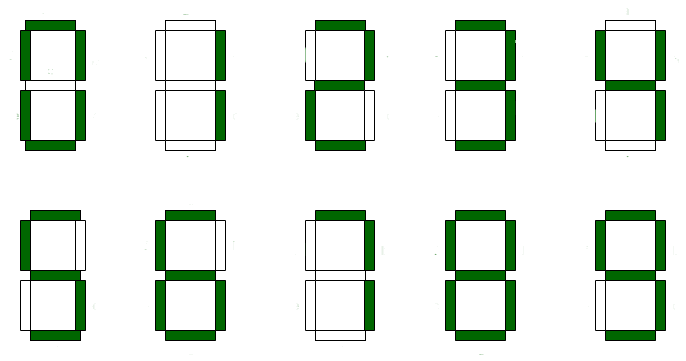
\includegraphics[width=0.5\textwidth]{7segment}
\caption*{seven-segment LED displays}
\end{figure}

1101 binary (13 decimal) (or, placed into groups of 3 binary digits, 001 101) is 15 in octal (1 x 8 + 5 x 1.) Notice that 001 binary is 1 octal and 101 binary is 5 octal - the binary values that are seen in the octal digits.\\

\newpage

\subsection*{Sexagesimal}

\begin{center}
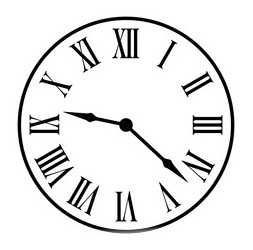
\includegraphics[width=0.5\textwidth]{old-fashion-vintage-clock-face}
\end{center}

Sexigesimal means based on 60s. The other number system that is commonly used around the world uses 60 as a base and is called the sexagesimal system. 60 is a very handy number to use because it divides evenly into so many other numbers – 30, 15, 20, 10, 5, 4, 3, and 2. It was first used by astronomers about three thousand years ago in the middle-east and it is why, among some other things, there are 24 hours in a day, 60 minutes to an hour, sixty seconds to a minute, and 360 degrees in a circle.
\newpage
\
\newpage
\
\newpage
\
\newpage
\
\newpage
\
\newpage
\
\newpage
\
\newpage
\

\begin{center}
\linespread{2}\large

Enquiries

\textbf{Applied Scholastics Ferndale}

Principal: Paula McLennan

mobile phone: 0431 683 306

email address: apsferndale@gmail.com

website: apsferndale.webs.com
\end{center}

\end{document}